\newsection
\section{Рабочий проект}
\subsection{Классы, используемые при разработке сайта}

можете выбрать следующий список классов и их методов, используемых при разработке веб-приложения (таблица 4.1).

\begin{longtable}[l]{|p{2cm}|p{2cm}|p{3.3cm}|p{6cm}|}
\caption{Описание классов, используемых в приложении\label{class:table}}\\
\hline \centering Название класса & \centering Модуль, к которому относится класс & \centering Описание класса &  Методы \\
\hline \centering 1 & \centering 2 & \centering 3 & 4\\
\endfirsthead
\caption*{Продолжение таблицы \ref{class:table}}\\
\hline \centering 1 & \centering 2 & \centering 3 & 4\\
\endhead

\hline string & Главный модуль & основной класс страницы веб-приложения. После одного из этапов загрузки страницы скрипт делает доступным инициализированный системой \$APPLICATION & string query = "INSERT INTO Usuarios (Nombre, Apellido, Email) VALUES (@Nombre, @Apellido, @Email)";
SqlCommand command = new SqlCommand(query, connection);

command.Parameters
.AddWithValue
("@Nombre", nombre);
command.Parameters
.AddWithValue
("@Apellido", apellido);
command.Parameters
.AddWithValue
("@Email", email);\\
\hline File & Главный модуль & File – Класс для работы с файлами и изображениями & Метод возвращает массив, содержащий описание файла (путь к файлу, имя файла, размер) с идентификатором\\
  \hline
\end{longtable}

\subsection{Тестирование разработанного web-сайта}

На рисунке \ref{main:image} представлена главная страница сайта «Программная система учёта процесса реабилитации животных в ветеринарной клинике».

\begin{figure}[H]
\center{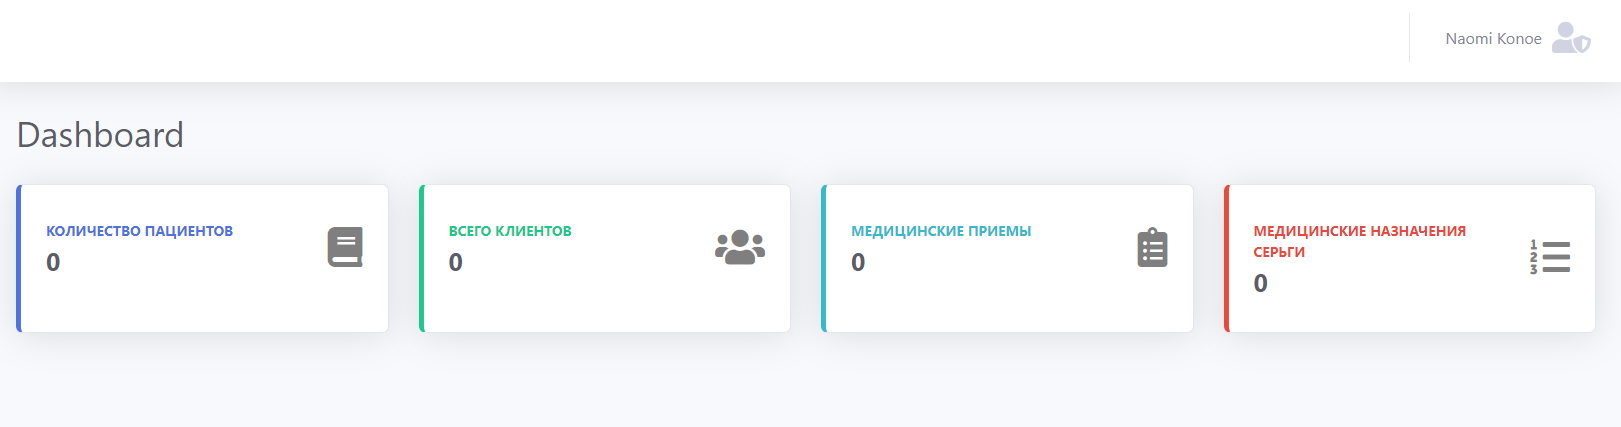
\includegraphics[width=1\linewidth]{Img 4}}
\center{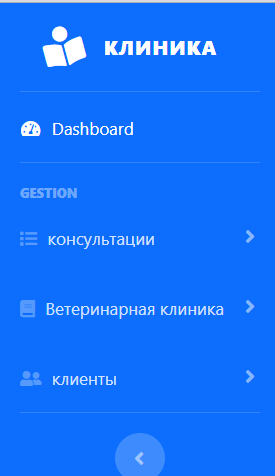
\includegraphics[width=0.5\linewidth]{Img 5}}
\caption{Главная страница сайта «Программная система учёта процесса реабилитации животных в ветеринарной клинике»}
\label{main:image}
\end{figure}

далее мы покажем схему базы данных, которую обрабатывает наше приложение, чтобы обеспечить максимальную производительность в работе


На рисунке \ref{menu:image} далее мы покажем схему базы данных, которую обрабатывает наше приложение, чтобы обеспечить максимальную производительность в работе.

\begin{figure}[H]
\center{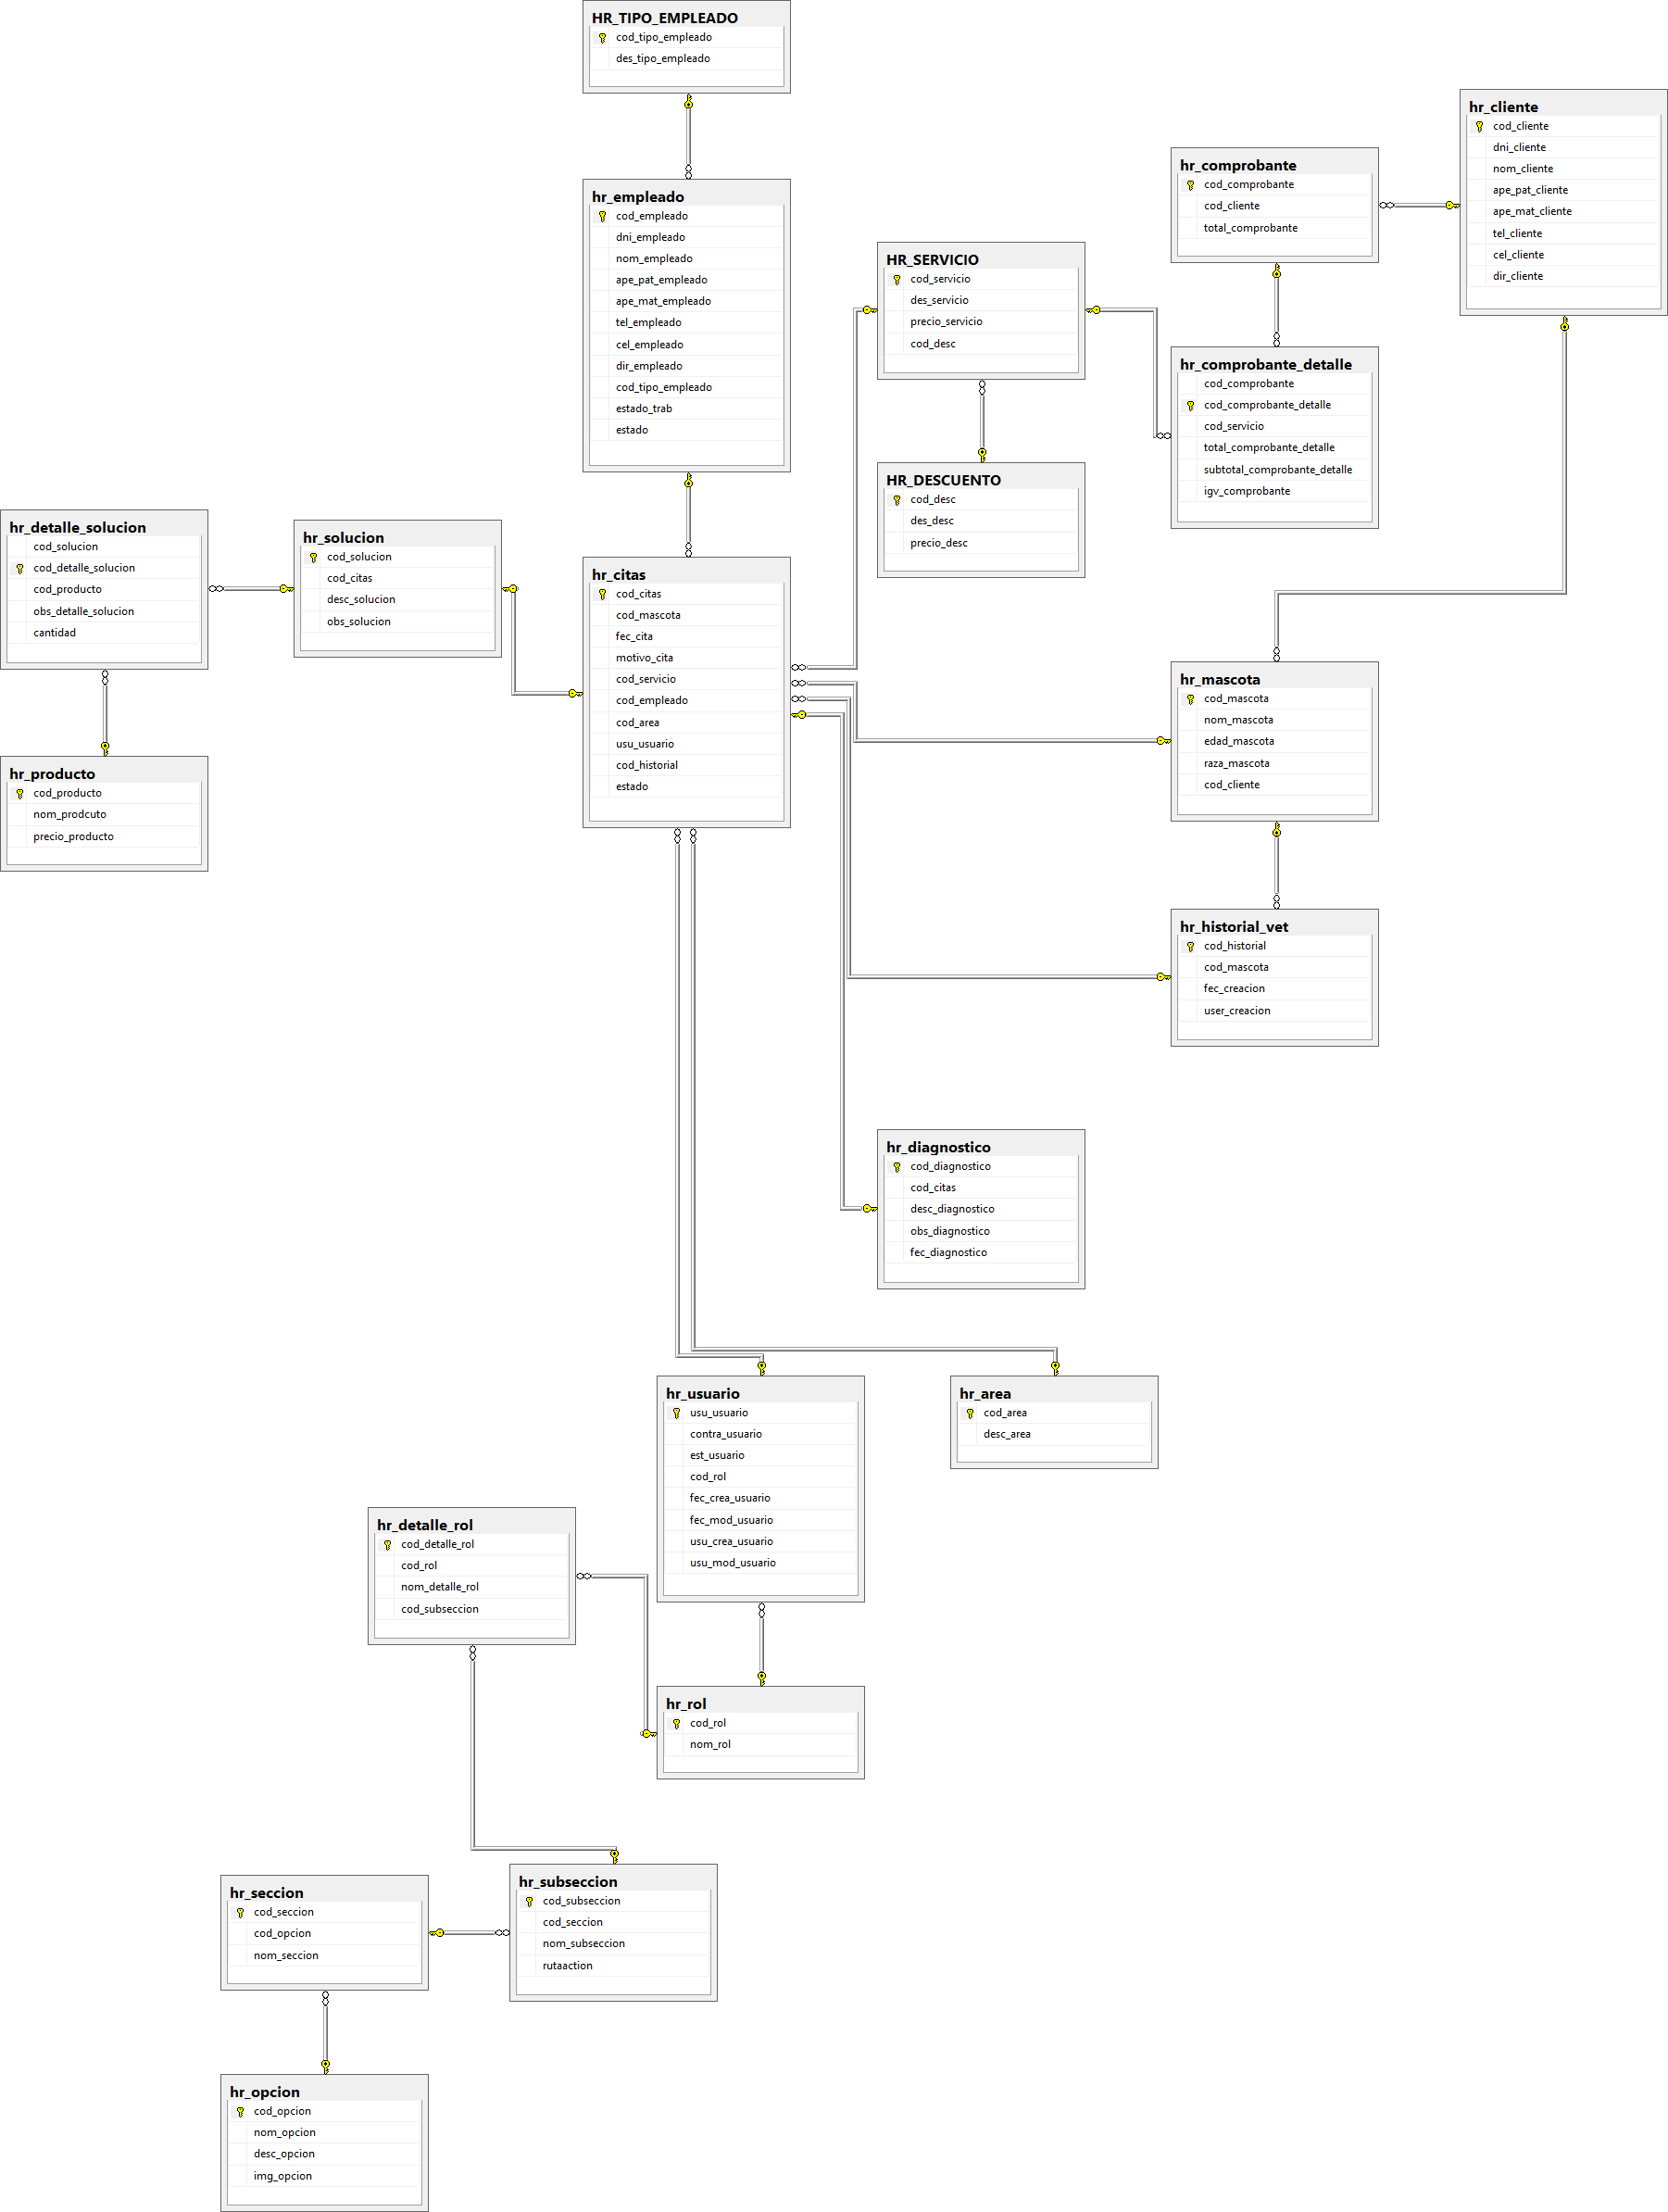
\includegraphics[width=0.7\linewidth]{Img 9}}
\caption{схема базы данных}
\label{menu:image}
\end{figure}

На рисунке 4.3 В этом разделе показаны отношения с базой данных в системе,.

\begin{figure}[H]
\center{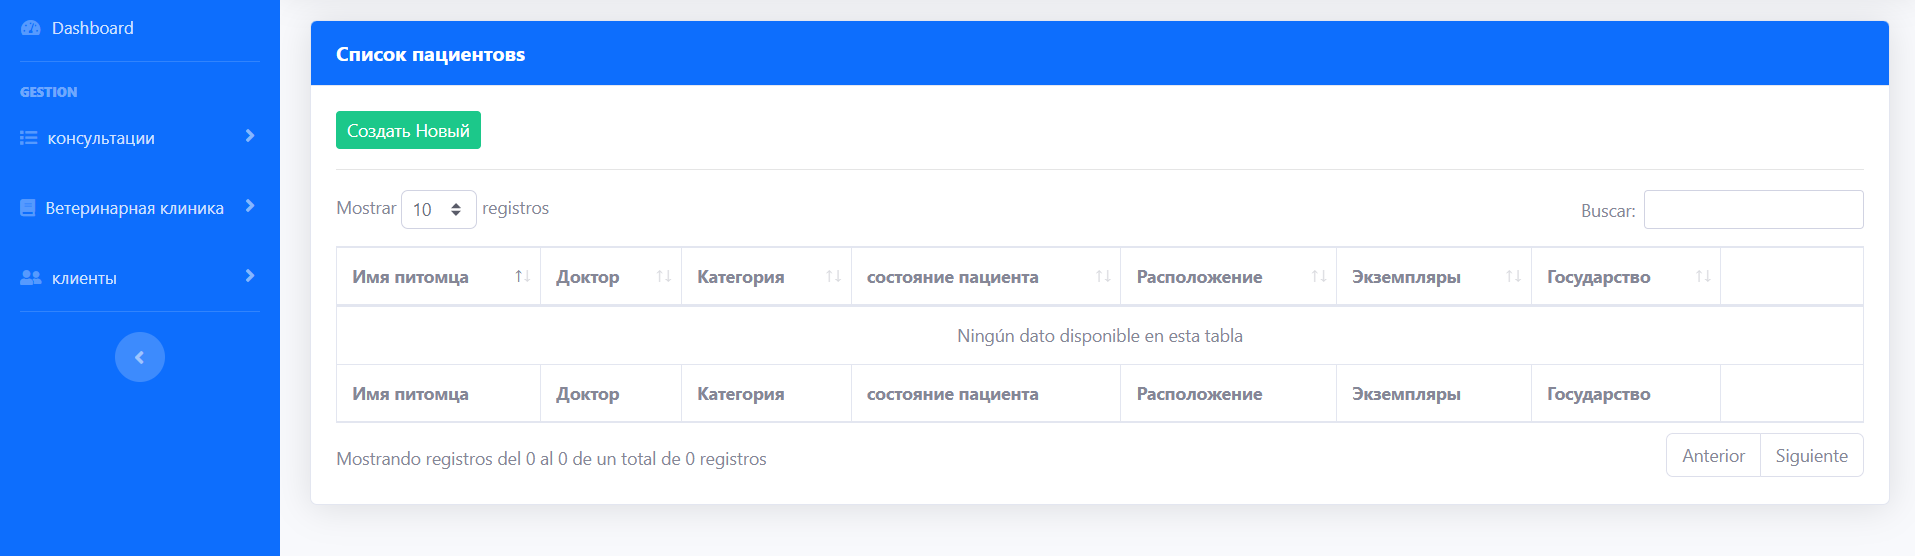
\includegraphics[width=1\linewidth]{Img 7}}
\caption{Динамический вывод заголовков}
\label{enter:image}	
\end{figure}

\begin{figure}[H]
	\center{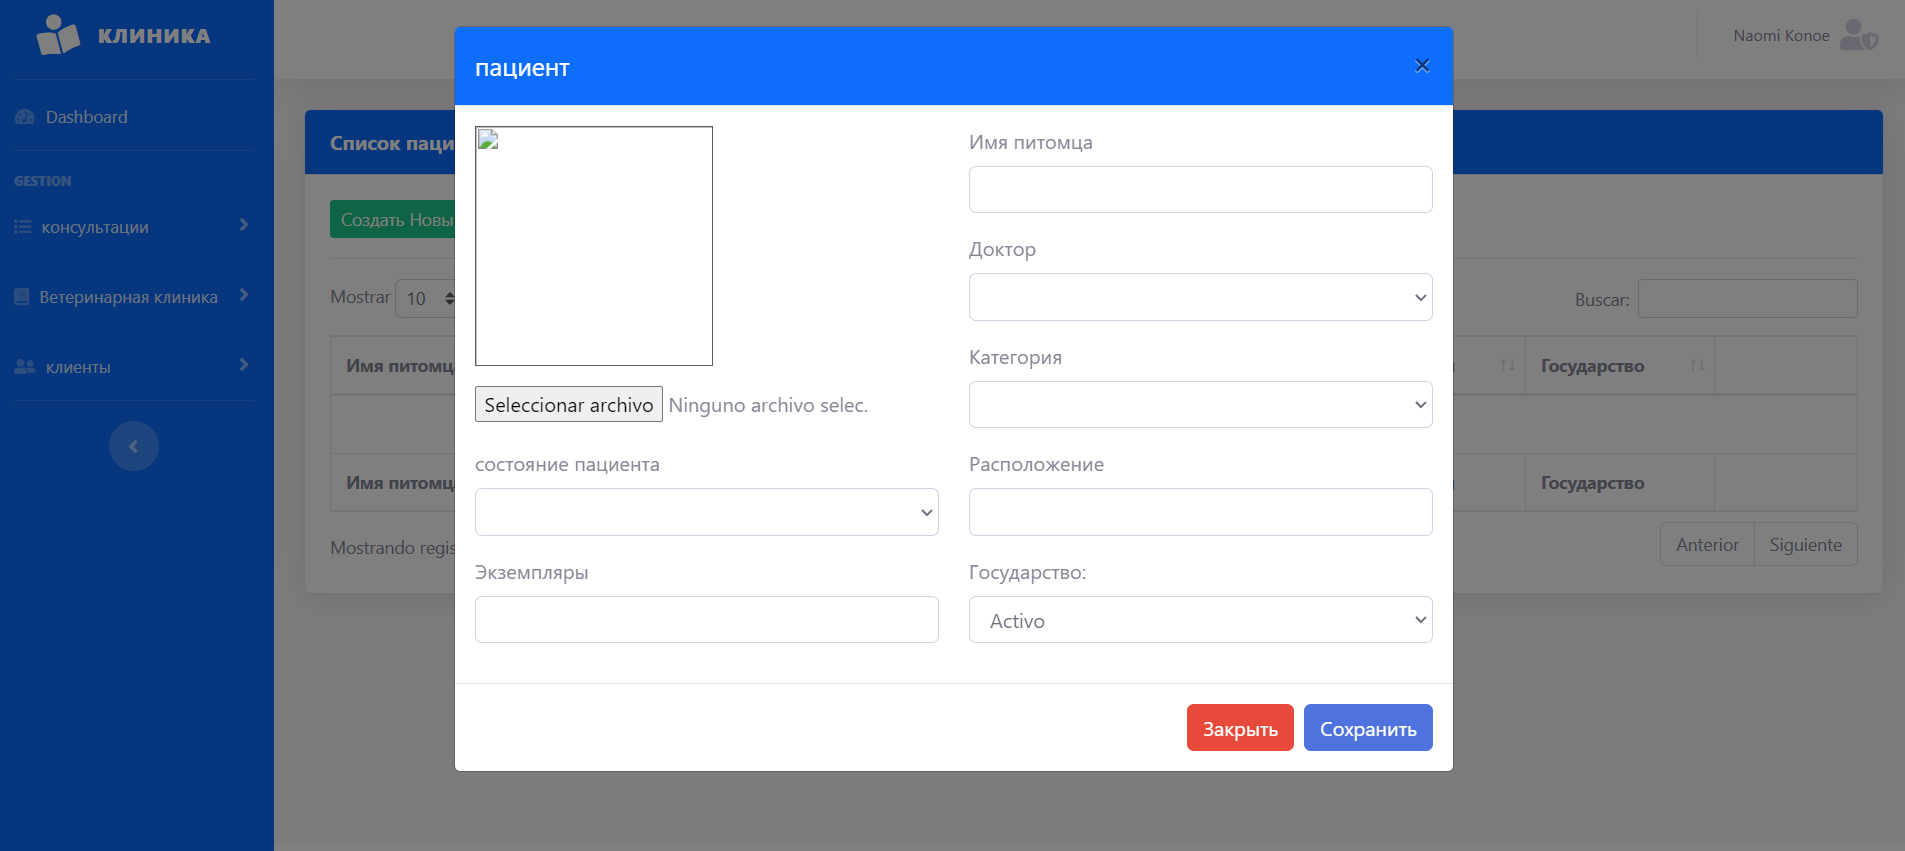
\includegraphics[width=1\linewidth]{Img 8}}
	\caption{Ввод данных для публикации очень-очень длинной, интересной и полезной}
	\label{enter:image}
\end{figure}
